% Reconciled hierarchy manuscript candidate.
% Source basis and incorporation custody are recorded separately in this project.
% Original ANF sections and Phases variants remain preserved, not required reading.
\documentclass[aps,prx,reprint,superscriptaddress,floatfix]{revtex4-2}
\usepackage{amsmath,amssymb,mathtools,bm,graphicx,booktabs,array,microtype}
\usepackage[colorlinks=true,linkcolor=blue,citecolor=blue,urlcolor=blue]{hyperref}
\hypersetup{pdftitle={Hierarchy in sampled collective feedback}}
\newcommand{\erf}{\operatorname{erf}}
\newcommand{\diag}{\operatorname{diag}}
\newcommand{\ran}{\operatorname{range}}
\newcommand{\E}{\mathbb E}
\begin{document}
\title{Hierarchy in sampled collective feedback}
\author{Gerard McCaul}
\date{\today}
\begin{abstract}
A collective can become better at detecting a small bias while becoming harder to control. Majority aggregation sharpens a population's mean response, but the dynamical consequence depends on where that response enters the feedback loop. We construct two sampled controllers and retain their full state. A functionally matched gradient controller has a fixed curve with transverse gain proportional to the square of the response slope. A post-observation response controller has an isolated equilibrium and a gain containing one response derivative. For the specified error-function models, the first admits a nonzero saddle cycle, whereas the second has a locally attracting symmetric cycle above its own threshold. Exact nested-majority trees then make hierarchy a calculable architectural choice. They can reduce gain at fixed size, but the admitted factorisations and finite block slopes matter. In the class of level-homogeneous odd-majority product trees, a positive lower-bound exponent prevents arbitrary-size gain suppression at fixed controller strength. A separate finite-horizon actuation problem supplies the other constraint: a terminal top displacement may be unreachable or costly, and requiring the lower levels to finish at rest can increase the minimum effort. The resulting feasible set is an intersection over specified architectures, controllers and intervention tasks, rather than a universal depth window. The derivations and retained finite examples distinguish local stability, finite transients and terminal effort without identifying any of them with a global dynamical phase.
\end{abstract}
\maketitle

\section{When a sharper collective response destabilises feedback}
\label{hrec:sec:problem}
Consider a detector array that repeatedly revises a common drive. Each detector returns a binary answer to a small signed signal. A positive majority asks for a positive correction, a negative majority for a negative one. Increasing the number of independent detectors makes the collective answer more decisive near the decision threshold. This is useful when the task is to distinguish two fixed alternatives. Once that answer changes the drive that generates the next observation, however, decisiveness becomes a feedback gain. The question is no longer only whether the detectors recognise a bias. It is whether the apparatus settles after they act on it.

A hierarchy changes this construction before it changes any differential equation. We can collect all detector outputs in one vote, or first form local majorities and then vote on their verdicts. Both arrangements use the same leaves. They do not have the same response curve. Nor does adding a level mean that we can move the resulting structure cheaply. An instruction applied at its base may need several updates to reach its top, and a prescribed final configuration can require cancellation of unwanted motion at intermediate levels. Static discrimination, closed-loop stability and the effort of an intervention are three questions about the same architecture. They require three explicit constructions.

This use of hierarchy is architectural rather than an assumption about institutional authority. Simon's definition encompasses interrelated subsystems nested within subsystems, and explicitly distinguishes that broader structure from a formal chain of command \cite{Simon1962236d85}. Feedback through an outcome that an intervention itself changes also has a precise contemporary formulation in performative prediction. There, the deployed predictor changes the distribution on which it is subsequently evaluated, and stability of retraining is distinct from risk optimality \cite{Perdomo2020a5b2ff}. Neither observation determines the gain of our detector array. To obtain that gain we must say what is aggregated, what the controller observes and when it acts.

We do this for two deterministic sampled models. One adjusts a broadcast by the gradient of a target response using an old report. The other first advances a relaxing plant, then applies a collective response to the newly observed mismatch. The placement of the response changes both the stability calculation and the nonlinear result. We then replace a flat detector bank by exact, specified majority trees, and finally attach an independently defined actuator. The contribution is the resulting chain of calculations: from a microscopic vote to its derivative, from that derivative to the appropriate full-loop boundary, and from an admitted architecture to a reachable intervention within budget. The derivations and numerical method are given below.


\section{The response generated by aggregation}
\label{hrec:sec:aggregation}
Let \(u\) be a broadcast signal and let the \(N\) detector outputs be \(\sigma_i\in\{-1,1\}\). Conditional on a fixed \(u\), assume they are independent with
\begin{equation}
 p(u)=\Pr(\sigma_i=1\mid u)=\frac{1+\tanh(\beta u)}2,\qquad \beta>0.
 \label{hrec:eq:detector}
\end{equation}
Here \(\beta\) has inverse-signal units. We define the collective response as the \emph{mean verdict}, the expected sign of the population vote:
\begin{equation}
 R_N^{\rm ex}(u)=\E\!\left[\operatorname{sign}\Bigl(\sum_{i=1}^N\sigma_i\Bigr)\,\middle|\,u\right].
 \label{hrec:eq:majority}
\end{equation}
For even \(N\), ties have expected verdict zero. A literal zero verdict and a fair binary tie-break have the same mean, but not the same variance or the same closure under further aggregation. We use odd blocks when constructing a nested binary hierarchy.

The slope at zero measures how strongly a small broadcast changes the expected vote. Differentiating a configuration probability at zero multiplies it by \(\beta\sum_i\sigma_i\). Consequently
\begin{align}
 G_N^{\rm ex}
 &=\bigl(R_N^{\rm ex}\bigr)'(0)=\beta\,\E|S_N|,\qquad S_N=\sum_i\sigma_i,\nonumber\\
 &=\beta N\,\frac{\binom{N-1}{\lfloor(N-1)/2\rfloor}}{2^{N-1}}.
 \label{hrec:eq:exact-slope}
\end{align}
Appendix~\ref{hrec:app:majority} derives the last equality. Its leading behaviour is \(\beta\sqrt{2N/\pi}\). The relative correction is \(+1/(4N)\) for odd \(N\) and \(-1/(4N)\) for even \(N\). Thus even the first correction remembers the actual finite voting rule.

For comparison, the arithmetic mean \(N^{-1}\sum_i\sigma_i\) has expectation \(\tanh(\beta u)\), whose origin slope is simply \(\beta\). Averaging and thresholding do different things. The average has variance \(1/N\) at zero bias, while an odd-population binary majority verdict has variance one. A steep \emph{mean} verdict is not a nearly noiseless single verdict. Throughout the dynamical calculations below, a response such as \(R_N\) is used deterministically as an expected control action. A physical implementation would need enough repeated samples, or an explicit stochastic model, to justify that replacement.

Two smooth responses will let us exhibit the controller distinction analytically:
\begin{equation}
 \begin{aligned}
 f_N(\theta)&=\erf\!\left(\sqrt{N/2}\sinh(\beta\theta)\right),\\
 R_N(u)&=\erf\!\left(\beta\sqrt{N/2}\,u\right).
 \end{aligned}
 \label{hrec:eq:proxies}
\end{equation}
The error function is \(\erf(v)=2\pi^{-1/2}\int_0^v e^{-t^2}\,dt\). Both origin slopes equal \(\beta\sqrt{2N/\pi}\), but the functions are not identical. We treat each as an exactly specified deterministic model, not as an exact finite-binomial response. A Gaussian approximation to physical majority blocks would additionally require control of the approximation at every block and of its derivative through the composition. The exact tree calculation in Sec.~\ref{hrec:sec:hierarchy} needs no such approximation.

\section{Closing the adaptive loop}
\label{hrec:sec:loop}
The first placement makes the population response part of a relaxing report. At integer update \(k\), let \(m_k\) be that report and \(\theta_k\) the broadcast. Let \(M(\theta)\) denote its stationary plant response and \(F(\theta)\) the response the controller expects. The lagged gradient-mismatch map is
\begin{align}
 m_{k+1}&=r m_k+(1-r)M(\theta_k),\nonumber\\
 e_k&=m_k-F(\theta_k),\nonumber\\
 \theta_{k+1}&=\theta_k+\alpha F'(\theta_k)e_k.
 \label{hrec:eq:lagged}
\end{align}
The parameter \(0\le r<1\) is the retained fraction of the old report. For an exponentially relaxing plant observed every \(T>0\) with relaxation time \(\tau>0\), \(r=e^{-T/\tau}\). We do not require the additional limit \(T\gg\tau\). The positive step \(\alpha\) has units \([\theta]^2/[m]^2\). With \(m\) held fixed, the last line is a gradient step on \(\tfrac12[m-F(\theta)]^2\), not gradient descent on an asserted global objective for the coupled system. Crucially, it uses \(m_k\), not \(m_{k+1}\).

Suppose \(M(\theta_*)=F(\theta_*)=m_*\), and write \(s=M'(\theta_*)\), \(b=F'(\theta_*)\). For \(C^2\) responses the equilibrium Jacobian in state order \((m,\theta)\) is
\begin{equation}
 J_{\rm lag}=
 \begin{pmatrix}r&(1-r)s\\ \alpha b&1-\alpha b^2\end{pmatrix}.
 \label{hrec:eq:lagged-jacobian}
\end{equation}
The linear mismatch obeys
\begin{equation}
 \delta e_{k+1}=(r-\alpha b^2)\delta e_k+(1-r)(s-b)\delta\theta_k.
 \label{hrec:eq:linear-mismatch}
\end{equation}
Point equality supplies an equilibrium. Equal slopes \(s=b\) additionally supply linear eigenvalues \(1\) and \(r-\alpha b^2\). They do not supply a family of equilibria. For example, \(M(\theta)=\theta+\theta^3\), \(F(\theta)=\theta\) match in value and slope at zero, yet their only intersection is zero. A fixed curve requires the stronger \emph{functional} identity \(M=F=f\) on a neighbourhood. In that case every \((f(\theta),\theta)\) is fixed, and the eigenvalue one represents motion tangent to that curve.

The second placement uses the detector population to convert a newly observed plant mismatch into a control action. Let \(x_k\) be a scalar plant state, let its stationary response be \(s\theta\), and let \(b\theta\) be the target, with \(b>s>0\). Using a positive response step \(\varepsilon\), define
\begin{align}
 x_{k+1}&=r x_k+(1-r)s\theta_k,\nonumber\\
 u_k&=x_{k+1}-b\theta_k,\nonumber\\
 \theta_{k+1}&=\theta_k+\varepsilon R_N(u_k).
 \label{hrec:eq:post}
\end{align}
Here \(R_N\) is dimensionless, \([\varepsilon]=[\theta]\), and \(s,b\) both have units \([x]/[\theta]\). Thus \(K=\varepsilon R_N'(0)\) has units \([\theta]/[x]\), and \(Kb\) is dimensionless. The sign convention makes a negative mismatch lower \(\theta\). For a strictly increasing odd \(R_N\), the only equilibrium is \((0,0)\): stationarity requires \(x=s\theta=b\theta\).

\begin{figure*}[t]
 \centering
 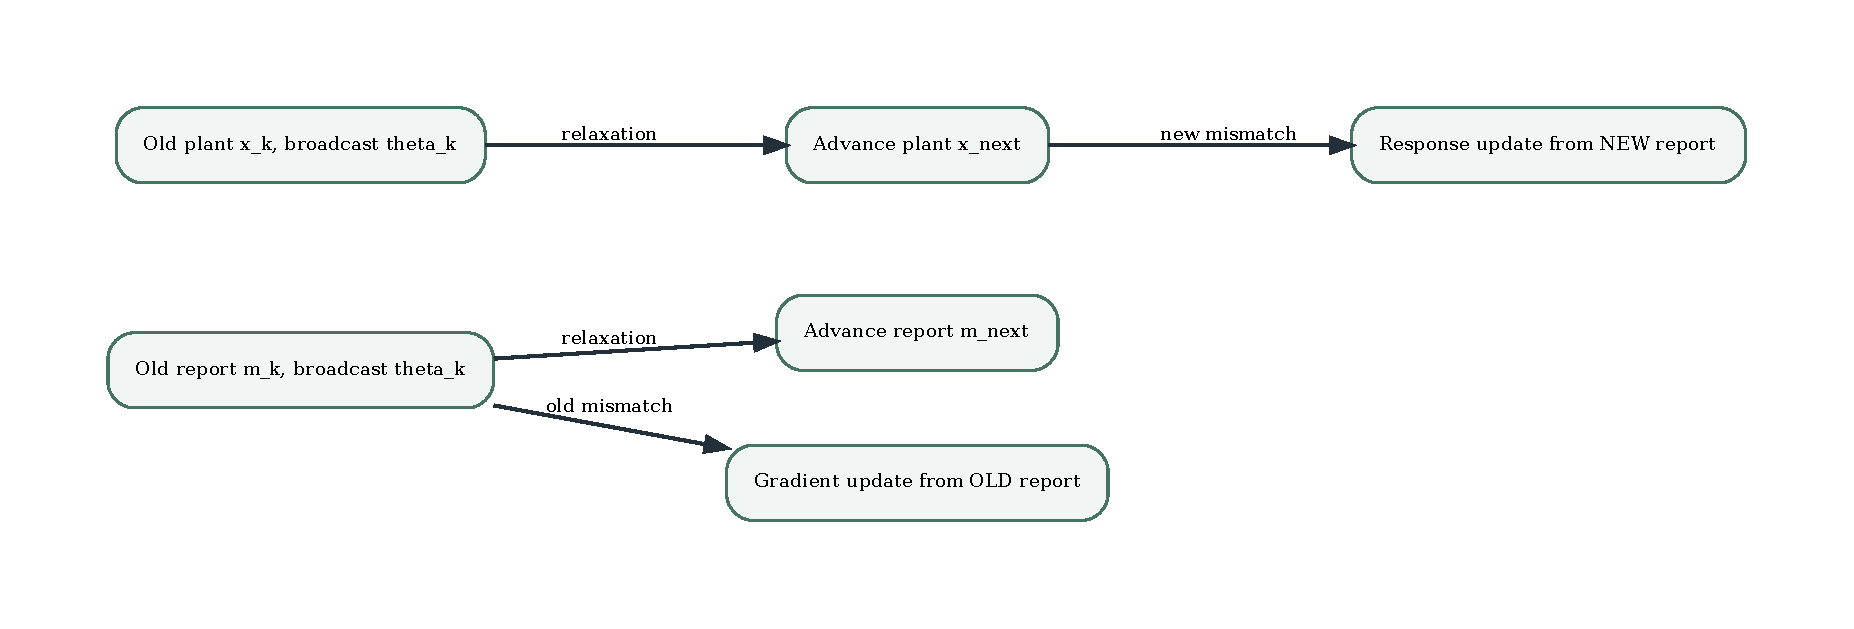
\includegraphics[width=\textwidth]{figures/generated/hierarchy-controller-timing-paper.pdf}
 \caption{The response must be located in time before its gain is calculated. In the lagged map, the plant advance and control update consume the old pair \((m_k,\theta_k)\). In the post-observation map, the plant advances first and its new state enters the response-driven update. The maps are Eqs.~\eqref{hrec:eq:lagged} and \eqref{hrec:eq:post}, respectively. Neither path is an elimination of the other.}
 \label{hrec:fig:timing}
\end{figure*}

Writing \(c_p=(1-r)s\), \(\Delta=b-c_p\) and \(K=\varepsilon R_N'(0)\), the second equilibrium Jacobian is
\begin{equation}
 J_{\rm post}(K)=
 \begin{pmatrix}r&c_p\\Kr&1-K\Delta\end{pmatrix}.
 \label{hrec:eq:post-jacobian}
\end{equation}
Only one response derivative enters \(K\). By contrast, functional matching in Eq.~\eqref{hrec:eq:lagged} gives the dimensionless transverse gain \(K_{\rm lag}=\alpha f'(\theta)^2\). The second derivative factor is not an extra population mechanism. It comes from choosing the target-gradient controller as well as a response-dependent plant. Figure~\ref{hrec:fig:timing} keeps this distinction visible.


\section{The finite-gain stability boundary}
\label{hrec:sec:stability}
For the matched lagged loop, the fixed curve is transversely linearly stable when
\begin{equation}
 |r-K_{\rm lag}|<1,\qquad K_{\rm lag}=\alpha f'(\theta)^2.
 \label{hrec:eq:transverse}
\end{equation}
At a nonzero-slope point this is \(0<K_{\rm lag}<1+r\). It is stability towards a curve, not asymptotic attraction to an isolated prescribed point. If \(\theta\) is externally frozen, the physical report update has only multiplier \(r\). The multiplier \(r-K_{\rm lag}\) belongs to the coupled loop.

The exact nonlinear mismatch makes the remaining state dependence explicit:
\begin{align}
 e_{k+1}&=r e_k-\{f(\theta_k+\alpha f'(\theta_k)e_k)-f(\theta_k)\}\nonumber\\
 &=A(\theta_k,e_k)e_k,\nonumber\\
 A(\theta,e)&=r-\alpha f'(\theta)\int_0^1
       f'(\theta+t\alpha f'(\theta)e)\,dt.
 \label{hrec:eq:secant}
\end{align}
This is a two-variable identity. It is not an autonomous cubic map for \(e\). At a strict stable point, continuity supplies a small rectangle on which \(|A|\le q<1\). If the initial mismatch is small enough that its accumulated broadcast drift remains inside that rectangle, \(|e_k|\le q^k|e_0|\) and \(\theta_k\) converges to some \(\theta_\infty\). Appendix~\ref{hrec:app:local} gives the explicit trapping condition. The result proves local attraction to the fixed curve. At equality in Eq.~\eqref{hrec:eq:transverse}, or for an arbitrary large excursion, this argument makes no assertion.

For the post-observation map, trace and determinant of Eq.~\eqref{hrec:eq:post-jacobian} give the three real two-dimensional Schur conditions. On \(b>s>0\), \(0\le r<1\), their nontrivial upper boundary is
\begin{equation}
 0<K<K_c,\qquad
 K_c=\frac{2(1+r)}{(1+r)b-(1-r)s}.
 \label{hrec:eq:post-boundary}
\end{equation}
At \(K=K_c\) one multiplier reaches \(-1\). The other lies in \([0,1)\), including zero when \(r=0\). This is not the matched fixed curve's simultaneous neutral and transverse boundary. The full conditions and the positive-slope off-matching lagged case appear in Appendix~\ref{hrec:app:local}.

These gains also give two different size laws. At the origin of the smooth responses in Eq.~\eqref{hrec:eq:proxies},
\begin{align}
 K_{\rm lag}(N)&=\frac{2\alpha\beta^2N}{\pi},
 &N_c^{\rm lag}&=\frac{\pi(1+r)}{2\alpha\beta^2},\nonumber\\
 K_{\rm post}(N)&=\varepsilon\beta\sqrt{\frac{2N}{\pi}},
 &N_c^{\rm post}&=\frac{\pi K_c^2}{2\varepsilon^2\beta^2}.
 \label{hrec:eq:size-laws}
\end{align}
The susceptibility exponent is \(1/2\) in both origin responses, but the \emph{gain} exponents are one and one half. For the lagged controls \(r=0.3,\alpha=0.01,\beta=0.5\), the origin transverse boundary is \(N_c^{\rm lag}=816.8140899\). The linear coefficient changes sign earlier at \(N_0=\pi r/(2\alpha\beta^2)=188.4955592\), where a small mismatch is cancelled to first order in one step. This is not a stability boundary. For \(b=1.2,s=0.4,r=e^{-1},\varepsilon=0.35,\beta=0.6\), the post-observation model instead has \(K_c=1.970146106\) and \(N_c^{\rm post}=138.2541437\).

What happens beyond a local boundary needs a nonlinear argument. For the matched erf/sinh map, a symmetric two-cycle with positive \(\theta\) satisfies
\begin{equation}
 \begin{aligned}
 m&=-\frac{1-r}{1+r}f(\theta),\\
 \alpha f'(\theta)f(\theta)&=(1+r)\theta.
 \end{aligned}
 \label{hrec:eq:matched-cycle}
\end{equation}
The full off-curve Jacobian is
\begin{equation}
 J(m,\theta)=
 \begin{pmatrix}
 r&(1-r)f'(\theta)\\
 \alpha f'(\theta)&1+\alpha f''(\theta)e-\alpha f'(\theta)^2
 \end{pmatrix}.
 \label{hrec:eq:full-jacobian}
\end{equation}
The \(f''e\) term matters. At a positive orbit state with \(f''<0\), \(e<0\) and
\(\det(I-J)=-\alpha(1-r)f''e<0\), so a real multiplier of \(J\) exceeds one. The retained \(N=900\) orbit has numerically evaluated two-step multipliers \(1.2451443679\) and \(0.5809714397\). It is a saddle, not an attracting phase branch.

The post-observation erf response supplies a positive contrast. Define \(D=b-(1-r)s/(1+r)\), so \(K_c=2/D\). Its symmetric orbit has broadcast amplitude \(\Theta>0\), plant amplitude \(X=-(1-r)s\Theta/(1+r)\), and mismatch magnitude \(z=D\Theta\). The orbit equation is
\begin{equation}
 \varepsilon\,\frac{R_N(z)}{z}=K_c.
 \label{hrec:eq:post-cycle}
\end{equation}
For an exact erf response, \(R_N(z)/z\) decreases strictly from \(R_N'(0)\) to zero. A unique positive symmetric solution therefore exists precisely when \(K>K_c\). Strict concavity gives \(0<\varepsilon R_N'(z)<K_c\). Both orbit Jacobians then satisfy the same strict Schur conditions as the equilibrium, proving local attraction of the two-cycle. Appendix~\ref{hrec:app:cycles} derives this result, including \(r=0\). It does not extend the conclusion to an arbitrary odd response or identify a global basin.

\begin{table}[t]
 \centering
 \caption{Finite trajectories of the matched erf/sinh loop. The initial state is \((m_0,\theta_0)=(10^{-4},0)\), with \(r=0.3,\alpha=0.01,\beta=0.5\). Peak means \(\max_{0\le k<H}|e_k|\), including the initial mismatch. Tail means half the range of \(e\) in the final 200 stored updates. Rounded values describe finite float64 observations, not exact asymptotic amplitudes.}
 \label{hrec:tab:transients}
 \begin{tabular}{rrrr}
 \toprule
 \(N\)&\(H\)&Peak&Tail\\
 \midrule
 800&5000&\(10^{-4}\)&roundoff scale\\
 817&5000&\(4.3872\,10^{-4}\)&not classified\\
 817&20000&\(1.93594\,10^{-2}\)&\(1.93601\,10^{-2}\)\\
 820&5000&\(9.37363\,10^{-2}\)&\(7.249\,10^{-5}\)\\
 850&5000&\(0.297630\)&roundoff scale\\
 900&20000&\(0.459980\)&roundoff scale\\
 \bottomrule
 \end{tabular}
\end{table}

Finite trajectories answer a different question from these orbit calculations. Table~\ref{hrec:tab:transients} separates the largest seeded excursion from a late-window amplitude. At \(N=900\), the peak occurs at update 123 and is followed by a small-mismatch tail. At \(N=817\), extending the horizon from 5000 to 20000 changes the peak by more than an order of magnitude, with the peak still at the final included sample. That case remains horizon-sensitive. Mirroring a nonnegative peak about zero would draw two apparent branches, but would not calculate a periodic orbit. Conversely, floating-point escape from the numerically initialised saddle does not remove the exact orbit of Eq.~\eqref{hrec:eq:matched-cycle}. The local theorem, orbit classification and finite observations retain their different jobs.


\section{What a specified hierarchy buys}
\label{hrec:sec:hierarchy}
Return to the detector array. Instead of voting once across all leaves, let each block form a binary majority and pass its verdict upward. Specify a level-homogeneous product tree
\(\mathcal T=(n_1,\ldots,n_L)\), with every span an odd integer at least three and
\(\prod_{\ell=1}^L n_\ell=N\). Conditional on a fixed broadcast, disjoint subtrees have independent binary outputs with the same distribution at each level. If \(B_n(v)\) is the mean majority verdict for independent and identically distributed (iid) inputs of mean \(v\), the successive means satisfy
\begin{equation}
 v_0(u)=\tanh(\beta u),\qquad
 v_\ell(u)=B_{n_\ell}(v_{\ell-1}(u)).
 \label{hrec:eq:tree}
\end{equation}
This conditional binary closure is what licenses composition. Its exact origin slope is
\begin{equation}
 \begin{aligned}
 G_{\mathcal T}&=\beta\prod_{\ell=1}^L a(n_\ell),\\
 a(n)&=n\binom{n-1}{(n-1)/2}2^{-(n-1)}.
 \end{aligned}
 \label{hrec:eq:tree-slope}
\end{equation}
It is a static derivative. Adding actual intermediate controllers or delays would require their states in a new dynamical model.

The distinction between amplification and attenuation is now concrete. A three-input majority has \(B_3(v)=(3v-v^3)/2\). Two such levels have slope \(9\beta/4\), smaller than the flat nine-input slope \(315\beta/128\), but larger than the individual slope \(\beta\). The hierarchy amplifies a leaf bias while attenuating the response \emph{relative to the flat architecture}. Relative attenuation need not bound the absolute gain as the population grows.

\begin{figure}[t]
 \centering
 \fbox{\begin{minipage}{0.91\columnwidth}
 \centering
 Nine iid binary leaves\\[5pt]
 \begin{tabular}{cc}
 Flat vote & Nested votes\\
 \(B_9\) & \(B_3\circ B_3\)\\[3pt]
 \(G/\beta=315/128\) & \(G/\beta=(3/2)^2=9/4\)
 \end{tabular}
 \end{minipage}}
 \caption{Hierarchy changes a response, not just a depth label. The two trees use the same nine iid leaves. Every internal block in the nested construction emits a binary verdict. The displayed exact derivatives are evaluated at zero broadcast. Smaller nested gain is relative to flat majority, not attenuation below the single-leaf sensitivity.}
 \label{hrec:fig:trees}
\end{figure}

Depth is also constrained by the leaves. In this class, \(L\le\lfloor\log_3N\rfloor\), and a depth is admitted only when the size factors into its allowed spans. For the explicit family \(N=3^k\), \(n_\ell=3^{j_\ell}\), the admissible level sequences are ordered compositions \(j_1+\cdots+j_L=k\) with positive \(j_\ell\). There are \(2^{k-1}\) sequences in total and \(\binom{k-1}{L-1}\) at depth \(L\). These are not all unbalanced trees on \(N\) leaves.

To place a tree in a controller, write its response as \(R_{\mathcal T}(u)=v_L(u)\). For the matched lagged comparison, replace both plant and target by \(M=F=R_{\mathcal T}\), evaluate the fixed-curve point at zero broadcast, and hold \(\alpha,r\) fixed. For the post-observation comparison, replace only \(R_N\) by \(R_{\mathcal T}\), holding the linear plant, target and response step fixed.

A retained exact-rational enumeration covers all 255 such sequences for \(k=1,\ldots,8\). To express their controller-specific gain tests in one notation, write
\begin{equation}
 \frac{K_{\mathcal T}}{K_c}
   =\eta\left(\frac{G_{\mathcal T}}{\beta}\right)^\nu,
 \qquad \eta>0.
 \label{hrec:eq:normalised-gain}
\end{equation}
The exponent \(\nu=1\) describes the post-observation placement, with \(\eta=\varepsilon\beta/K_c\). The exponent \(\nu=2\) describes the matched gradient placement at zero broadcast, with \(\eta=\alpha\beta^2/(1+r)\) and transverse threshold \(K_c=1+r\). Thus each prefactor retains its controller's own threshold. At the illustrative control \(\eta=1/8,\nu=1\), a slope \(G_{\mathcal T}/\beta<8\) is required. At \(N=243\), the flat slope is \(12.4505920090\), but the all-three depth-five slope is \(243/32=7.59375\). Exactly one of the 16 admitted level sequences meets the strict gain test. At \(N=729\), even the smallest attained slope, \(729/64=11.390625\), exceeds eight. None of its 32 sequences qualifies. A hierarchy can rescue a finite case without providing unlimited rescue.

There is an analytic obstruction for this entire odd-product class, not merely for those enumerated sizes. The exact block slopes satisfy
\begin{equation}
 a(n)\ge\sqrt{\frac{n+1}{2}}>\sqrt{\frac n2},
 \qquad n\ge3\ \text{odd}.
 \label{hrec:eq:block-bound}
\end{equation}
Using \(L\le\log_3N\) gives
\begin{equation}
 G_{\mathcal T}>\beta\sqrt N\,2^{-L/2}
 \ge\beta N^\gamma,\qquad
 \gamma=\frac{1-\log_3 2}{2}>0.
 \label{hrec:eq:tree-bound}
\end{equation}
At fixed positive controller strength, selecting more levels in this class cannot keep the local gain bounded for arbitrarily large \(N\). Appendix~\ref{hrec:app:depth} proves the block inequality by a recurrence. Fair-tie binary trees, arbitrary unbalanced trees and correlated leaves are not members of this theorem's class.

A convenient abstract depth law remains useful when it is actually available. Suppose, on a specified starting domain and admitted size set,
\begin{equation}
 \begin{gathered}
 K(N,L)=K_{\rm ref}(N/N_{\rm ref})^p d^{L-1},\\
 K_{\rm ref}>0,\qquad p>0,\qquad 0<d<1.
 \end{gathered}
 \label{hrec:eq:depth-law}
\end{equation}
Here \(p\) is the total \emph{gain} exponent and \(d\) the per-level gain attenuation. Solving \(K=K_c\) gives
\begin{equation}
 N_c(L)=N_{\rm ref}
 \left(\frac{K_c}{K_{\rm ref}}\right)^{1/p}
 d^{-(L-1)/p}.
 \label{hrec:eq:critical-size}
\end{equation}
The reciprocal \(p\) cannot be dropped. If a level attenuates the response slope by \(q\), a controller containing \(\nu\) such derivatives has \(d=q^\nu\). A fixed Gaussian-block approximation suggests a response factor \((2/\pi)^{(L-1)/2}\) relative to flat majority, but applying it repeatedly to small blocks without error control is not the exact tree law. In particular, the Gaussian depth-six proxy can predict a subcritical \(N=729\) while the exact depth-six all-three tree still fails the test.

For integer \(L\), strict stability in Eq.~\eqref{hrec:eq:depth-law} requires
\begin{equation}
 L_{\min}=\max\left\{1,\,
 2+\left\lfloor
 \frac{\log[K_{\rm ref}(N/N_{\rm ref})^p/K_c]}{\log(1/d)}
 \right\rfloor\right\}.
 \label{hrec:eq:integer-floor}
\end{equation}
This includes the equality case: gain exactly at threshold requires another level. It is only a candidate depth until intersected with the architecture's admitted factorisations. If the gain exponent is zero, the finite prefactor decides which side of the boundary the system occupies. If it is negative, the gain can eventually fall below the boundary while still exceeding it at smaller admitted sizes. Neither sign by itself establishes criticality or all-size stability.


\section{The cost of moving a deep structure}
\label{hrec:sec:actuation}
The gain calculation describes a response to a held broadcast. It does not say how an instruction moves through the physical structure. We therefore specify an actuator separately. Let \(z_t\in\mathbb R^L\), let \(e_i\) denote the coordinate basis vectors, and let \(S\) have ones on its first subdiagonal and zeros elsewhere. The base is coordinate one and the top is coordinate \(L\). For \(t=0,\ldots,H-1\), take
\begin{equation}
 \begin{gathered}
 z_{t+1}=A z_t+B v_t,\\
 A=aI+cS,\qquad B=g e_1.
 \end{gathered}
 \label{hrec:eq:chain}
\end{equation}
The persistence \(a\), transmission \(c\) and actuator gain \(g\) are specified properties of this model. A pure shift has \(a=0\). A persistent chain has \(a\ne0\), with \(a=1\) allowing local accumulation. The shift is not a chain of unit integrators.

An intervention task also needs an initial state \(z_0\), an integer horizon \(H\), a target and a cost metric. In chronological input order \(\bm v=(v_0,\ldots,v_{H-1})^\top\),
\begin{equation}
 \begin{gathered}
 z_H=A^H z_0+C_H\bm v,\\
 C_H=[A^{H-1}B,\ldots,AB,B].
 \end{gathered}
 \label{hrec:eq:chronological}
\end{equation}
A full terminal target \(z_*\) requires defect \(q=z_*-A^Hz_0\). A scalar top target \(e_L^\top z_H=\delta\) requires only
\(d_y=\delta-e_L^\top A^Hz_0\), leaving other terminal components free. Effort is
\begin{equation}
 J=\bm v^\top R_H\bm v,\qquad R_H\ \text{positive definite}.
 \label{hrec:eq:effort}
\end{equation}
For the uniform metric \(R_H=wI\), state units \(Z\), input units \(U\), \([g]=Z/U\) and \([w]=\text{effort}/U^2\). The reference \(E_0=w\delta^2/g^2\) has the chosen effort units. Those units are not necessarily joules. A terminal squared-input task does not become heat dissipation or sustained maintenance by renaming its cost.

Reachability comes before minimisation. Put \(\mathcal M=C_H\), \(b_q=q\) for a full target, or \(\mathcal M=e_L^\top C_H\), \(b_q=d_y\) for the top output. If \(b_q\notin\ran(\mathcal M)\), the exact task is infeasible and its extended minimum is \(+\infty\). If it is reachable, whitening by \(R_H^{1/2}\) gives the unique optimum
\begin{align}
 \bm v_*&=R_H^{-1}\mathcal M^\top
       (\mathcal M R_H^{-1}\mathcal M^\top)^+b_q,\nonumber\\
 J_{\min}&=b_q^\top(\mathcal M R_H^{-1}\mathcal M^\top)^+b_q.
 \label{hrec:eq:min-effort}
\end{align}
The superscript \(+\) denotes the Moore--Penrose pseudoinverse. It is not a substitute for the reachability condition. An unreachable top direction can have zero pseudoinverse quadratic, which is not zero effort to reach it.

The chain's impulse response follows from the commuting terms \(aI\) and \(cS\):
\begin{equation}
 A^jB=g\sum_{i=0}^{\min(j,L-1)}
       \binom ji a^{j-i}c^i e_{i+1}.
 \label{hrec:eq:impulse}
\end{equation}
For \(gc\ne0\), the first \(\min(H,L)\) power columns are triangular with nonzero successive diagonal entries \(gc^j\), so \(\operatorname{rank}C_H=\min(H,L)\). Starting from zero, a nonzero top target is unreachable for \(H<L\), however large the input budget.

For a pure shift, only \(v_{H-L}\) can reach the top at time \(H\). When \(H\ge L\), choosing \(v_{H-L}=\delta/(gc^{L-1})\) and all other inputs zero gives
\begin{equation}
 J_{\rm top}=E_0c^{-2(L-1)}.
 \label{hrec:eq:shift-cost}
\end{equation}
It also makes all lower terminal components zero. Thus the scalar top and full pure-apex targets \(z_*=\delta e_L\) have identical cost in this special case. Extra time beyond \(L\) gives no further reduction, because the shift's finite-horizon Gramian has already saturated.

Persistence changes both conclusions. Consider \(L=2,a=1,c=1/2,g=w=1,z_0=0\), with top target one. At \(H=2\), the chronological scalar-optimal input \((2,0)\) leaves \(z_2=(2,1)\), at cost four. To finish instead at the pure apex \((0,1)\), the input must be \((2,-2)\), at cost eight. The extra input cancels the lower terminal component. The scalar solution is cheaper because it solves a less restrictive task, not because it finds a better solution to the same full-state problem. At \(H=3\), the scalar control is \((0.8,0.4,0)\), with cost \(4/5\), whereas \((1,0,-1)\) reaches the pure apex with cost two.

\begin{figure}[t]
 \centering
 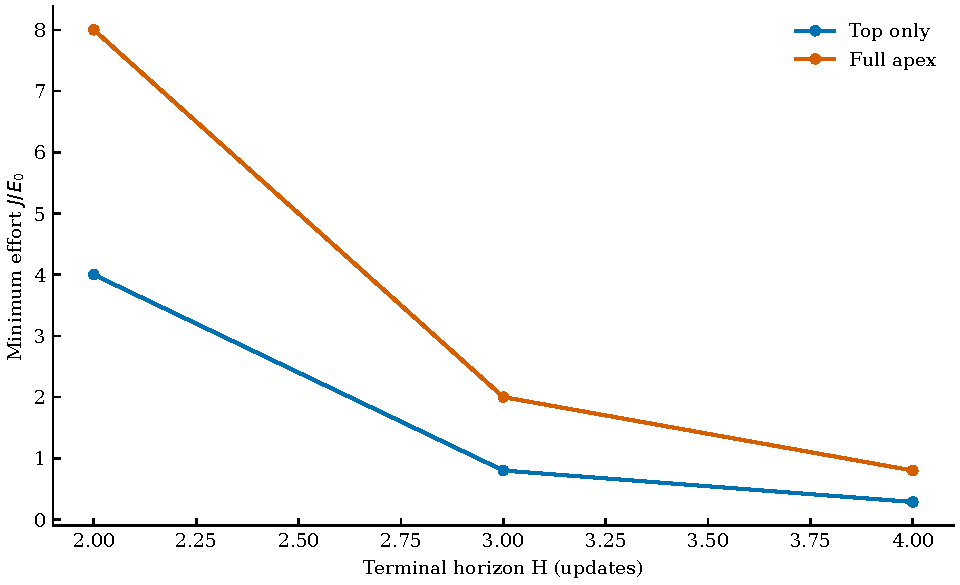
\includegraphics[width=\columnwidth]{figures/generated/persistent-terminal-effort-paper.pdf}
 \caption{Time helps according to the terminal task. Retained numerical optima for the two-state persistent chain \(a=1,c=1/2,g=w=1,z_0=0\). The top-only target is \(z_2(H)=1\). The full-apex target additionally requires \(z_1(H)=0\). Only the declared horizons \(H=2,3,4\) are plotted, with lines joining these samples as visual guides. At \(H=1\), both nonzero top tasks are unreachable, not zero-cost. The normalisation is \(E_0=1\) in illustrative squared-input units. No calibrated physical energy or uncertainty model is implied.}
 \label{hrec:fig:effort}
\end{figure}

The horizon theorem has an equally definite scope. For zero initial state, a fixed terminal target and uniform positive metric, minimum full-state effort is nonincreasing as \(H\) grows. With \(W_H=C_HC_H^\top\), full rank holds for \(H\ge L\). Writing \(v_H=A^HB\), Sherman--Morrison gives
\begin{equation}
 J_H-J_{H+1}
 =\frac{w(q^\top W_H^{-1}v_H)^2}
        {1+v_H^\top W_H^{-1}v_H}\ge0.
 \label{hrec:eq:horizon}
\end{equation}
Improvement is strict only when the numerator is nonzero. In the same two-state chain, the \emph{different} full target \(q=(6,1)^\top\) has effort 20 at both \(H=2\) and \(H=3\). For top-only targets, every extra impulse-response term is positive when \(a\ne0\), so effort decreases strictly once \(H\ge L\). Appendix~\ref{hrec:app:control} proves these claims and covers singular reachable cases.

We can now combine the two constructions without conflating their coefficients. Let \(\mathcal A(N)\) be the admitted architecture set, and assign to each architecture its actual controller gain and its specified actuation model. Then
\begin{equation}
 \mathcal F(N)=\left\{\mathcal T\in\mathcal A(N):
 \begin{array}{l}
 0<K_{\mathcal T}<K_c,\\
 b_q\in\ran(\mathcal M_{\mathcal T,H}),\\
 J_{\min}(\mathcal T,H)\le E_{\max}
 \end{array}\right\}.
 \label{hrec:eq:feasibility}
\end{equation}
The inequality refers to the corresponding controller's local criterion. It does not certify a global attractor. Static gain attenuation \(d\) and actuator transmission \(c\) enter different calculations. A relation such as \(d=c^2\) would be an additional coupling hypothesis, not a consequence of reversing a many-to-one majority map.

A simple depth window is a conditional specialisation of Eq.~\eqref{hrec:eq:feasibility}. For the zero-initial-state shift task, \(0<c<1\), \(H\ge1\), and \(E_{\max}/E_0\ge1\),
\begin{equation}
 L\le L_{\rm cap}=\min\left\{H,\,
 1+\left\lfloor\frac{\log(E_{\max}/E_0)}{\log(c^{-2})}\right\rfloor\right\}.
 \label{hrec:eq:budget-cap}
\end{equation}
If all integer depths from one to \(L_{\rm cap}\) are admitted and Eq.~\eqref{hrec:eq:depth-law} is valid, feasibility reduces to \(L_{\min}(N)\le L_{\rm cap}\). Its size bound is the strict supremum
\begin{equation}
 N<N_{\rm sup}=N_{\rm ref}(K_c/K_{\rm ref})^{1/p}
 d^{-(L_{\rm cap}-1)/p}.
 \label{hrec:eq:conditional-size}
\end{equation}
The budget allows equality, whereas stability does not. Actual product-tree sizes must still be intersected with their admitted set. Persistent chains generally require the task-specific Gramian rather than this shift-only ceiling.


\section{Measuring the feedback regime}
\label{hrec:sec:consequence}
For the detector array, the calculation suggests a direct order of measurement. Hold the broadcast fixed and estimate the mean response to a small perturbation, including its conditional dependence across detectors. Specify whether the recorded signal is an average, a binary verdict or an average over repeated verdicts. Next measure the plant's relaxation over the actual sampling period and record the controller's update law. An old report multiplied by a target gradient and a new report passed through a majority response are not interchangeable observations of the same gain. Their different Jacobians are testable statements about timing and local response.

An intervention requires another specification. Choose the initial condition, the horizon, the target components and the physical input metric before quoting a cost. In the two-state example, allowing the lower terminal state to remain nonzero halves the \(H=2\) effort. That difference cannot be inferred from the static vote slope. A claim that one microscopic coefficient controls both the aggregation response and the actuation transmission would need an independently justified architectural model or measurement.

The construction therefore gives a practical architecture test. Hierarchy can be designed as a response transformation and tested against a controller-specific stability condition. Exact product trees make that test finite and reproducible: the \(243\)-leaf example gains an admissible subcritical architecture, while the \(729\)-leaf example does not. Reachability and minimum-norm control then price a declared intervention on a separately specified chain. These calculations replace an unrestricted depth prescription by the feasible set in Eq.~\eqref{hrec:eq:feasibility}.

What remains open is also specific. The local fixed-curve theorem does not decide the global fate of the matched loop, and the \(817\)-control trajectory is unresolved at its retained horizon. The post-observation cycle theorem identifies a local attractor, not its global basin. General unbalanced or correlated aggregation architectures need their own response calculations. A physical identification of static attenuation with actuator transmission has not been established here. None of these questions erases the finite rescue, the odd-tree lower bound or the terminal cancellation mechanism. They identify which next inference needs more than the constructions already given.


\appendix
\section{Exact majority response}
\label{hrec:app:majority}
With \(p=(1+v)/2\), the mean-majority polynomial is
\begin{equation}
 B_N(v)=\sum_{j=0}^N
 \operatorname{sign}(2j-N)\binom Nj p^j(1-p)^{N-j}.
\end{equation}
At \(u=0\), each spin configuration has probability \(2^{-N}\). Differentiation using Eq.~\eqref{hrec:eq:detector} multiplies that probability by \(\beta S_N\), giving the first line of Eq.~\eqref{hrec:eq:exact-slope}. For the binomial sum, use
\[
 (2j-N)\binom Nj
 =N\left[\binom{N-1}{j-1}-\binom{N-1}j\right].
\]
Summing over \(j>N/2\) telescopes. Doubling the positive contribution by symmetry yields
\(\E|S_N|=N2^{-(N-1)}\binom{N-1}{\lfloor(N-1)/2\rfloor}\).
A tie contributes zero to this derivative.

For \(N=2j\), Stirling expansion of the central binomial coefficient gives
\(\E|S_N|=\sqrt{2N/\pi}[1-1/(4N)+O(N^{-2})]\).
For \(N=2j+1\), the corresponding expansion has \(+1/(4N)\).
For even \(N\), the literal-zero tie rule has variance
\(1-\Pr(S_N=0)\) at zero bias, while a fair binary tie-break has variance one. Their equal mean laws therefore do not license an identical binary stochastic recursion.


\section{Full-loop local stability}
\label{hrec:app:local}
Differentiating Eq.~\eqref{hrec:eq:lagged} at zero mismatch removes the \(F''e\) term and gives Eq.~\eqref{hrec:eq:lagged-jacobian}. Subtracting \(b\delta\theta_{k+1}\) from \(\delta m_{k+1}\) gives Eq.~\eqref{hrec:eq:linear-mismatch} directly, without eliminating either state. If \(F'\ne0\) throughout a neighbourhood, a fixed point satisfies \(m=M(\theta)\) from the plant and \(m=F(\theta)\) from the controller. Hence the entire graph is fixed precisely when \(M=F\) there. Zeros of \(F'\) can supply additional stationary points and must be treated separately.

For \(b>s>0\), the lagged trace and determinant are
\[
 t=1+r-\alpha b^2,\qquad
 \delta=r-\alpha r b^2-\alpha(1-r)bs.
\]
The Schur expressions are
\begin{align*}
 1-t+\delta&=\alpha(1-r)b(b-s)>0,\\
 1+t+\delta&=2(1+r)-\alpha[(1+r)b^2+(1-r)bs],\\
 1-\delta&=1-r+\alpha[rb^2+(1-r)bs]>0.
\end{align*}
Thus strict local linear stability is equivalent to
\[
 0<\alpha<
 \frac{2(1+r)}{(1+r)b^2+(1-r)bs}.
\]
At \(b=s\), the first Schur expression vanishes and an eigenvalue is one. This fact alone gives no nonlinear family.

For the post-observation map, the trace and determinant are
\(t=1+r-K\Delta\), \(\delta=r(1-Kb)\). The three expressions become
\begin{align*}
 1-t+\delta&=K(1-r)(b-s),\\
 1+t+\delta&=2(1+r)-K[(1+r)b-(1-r)s],\\
 1-\delta&=1-r+rKb.
\end{align*}
They prove Eq.~\eqref{hrec:eq:post-boundary}. At the upper boundary the companion multiplier is
\[
 \lambda_{\rm other}
 =r\,\frac{(1+r)b+(1-r)s}{(1+r)b-(1-r)s}.
\]
The denominator minus \(r\) times its numerator is
\((1-r)(1+r)(b-s)>0\), proving \(\lambda_{\rm other}<1\).
It is zero at \(r=0\).

For completeness, the matched loop has a nonlinear local attraction theorem. Let \(f\in C^2(U)\), with \(U\) an open interval, and suppose
\(|r-\alpha f'(\theta_*)^2|<1\).
Choose \(q\) strictly between this modulus and one. Continuity of the secant coefficient in Eq.~\eqref{hrec:eq:secant} supplies \(\rho,\epsilon>0\) such that \(I=[\theta_*-\rho,\theta_*+\rho]\subset U\), all required update segments remain in \(U\), and \(|A(\theta,e)|\le q\) for \(\theta\in I,|e|\le\epsilon\). Let \(M_f>0\) bound \(|f'|\) on \(I\). Initial conditions satisfying
\[
 \begin{gathered}
 |\theta_0-\theta_*|\le\rho/2,\\
 |e_0|<\min\{\epsilon,\rho(1-q)/(2\alpha M_f)\}.
 \end{gathered}
\]
remain in the tube. Indeed \(|e_k|\le q^k|e_0|\), while the sum of the broadcast increments is bounded by
\(\alpha M_f|e_0|/(1-q)<\rho/2\).
Induction keeps the whole trajectory in the rectangle. The increments are summable, so \(\theta_k\to\theta_\infty\in I\) and
\[
 |\theta_\infty-\theta_k|
 \le\frac{\alpha M_f|e_0|q^k}{1-q},\qquad
 m_k\to f(\theta_\infty).
\]
The required uniform secant bound is stronger than checking a finite list of instantaneous linear gains along a large excursion.

\section{The two symmetric cycles}
\label{hrec:app:cycles}
For the matched odd response, impose the orbit
\((m,\theta)\mapsto(-m,-\theta)\).
The plant equation gives the first identity in Eq.~\eqref{hrec:eq:matched-cycle}, and the controller gives the second. For the erf/sinh response, if
\(\alpha f'(0)^2>1+r\), the function
\(h(\theta)=\alpha f'(\theta)f(\theta)-(1+r)\theta\)
is positive for small positive \(\theta\) and negative eventually, since \(f'f\to0\). Continuity supplies a positive root, without asserting global uniqueness.

At a symmetric pair \(f'\) is even, while \(f''\) and \(e\) are odd, so both exact one-step Jacobians in Eq.~\eqref{hrec:eq:full-jacobian} coincide. Their characteristic polynomial at one is
\(\det(I-J)=-\alpha(1-r)f''e\).
If this is negative, the monic polynomial must cross zero at a real argument greater than one. To inspect the sign for the stated proxy, put \(v=\sqrt{N/2}\sinh(\beta\theta)\). Then
\[
 \begin{aligned}
 f''&=\frac{2e^{-v^2}}{\sqrt\pi}\,[v''-2v(v')^2],\\
 v''-2v(v')^2&=\beta^2v[1-N\cosh^2(\beta\theta)].
 \end{aligned}
\]
At \(N=900,\theta>0\), this is negative. The retained root is
\(\theta=0.025471791723687645\), \(m=-0.16024794040085039\).
Both directed map residuals are about \(2.78\,10^{-17}\). Direct multiplication of the two Jacobians gives the two-step multipliers quoted in the main text. Their decimal values are floating evaluations, not certified interval bounds.

For the post-observation orbit, the plant equation gives
\(X=-(1-r)s\Theta/(1+r)\), so the signed newly observed mismatch at the positive-\(\Theta\) state is \(-D\Theta\). Oddness reduces the control equation to
\(2\Theta=\varepsilon R_N(D\Theta)\), which is Eq.~\eqref{hrec:eq:post-cycle}.
Writing \(R_N(z)=\erf(\kappa z)\), \(\kappa=\beta\sqrt{N/2}>0\), gives \(R_N'>0\), \(R_N''<0\) for \(z>0\). Therefore
\[
 \begin{gathered}
 R_N(z)=\int_0^zR_N'(t)\,dt>zR_N'(z),\\
 \frac{d}{dz}\frac{R_N(z)}z<0.
 \end{gathered}
\]
The ratio decreases continuously from \(R_N'(0)\) to zero. This proves existence and uniqueness within the symmetric ansatz when \(K>K_c\), and nonexistence of a nonzero symmetric solution for \(K\le K_c\). At the orbit put \(k=\varepsilon R_N'(z)\). The inequality above gives \(0<k<K_c\). Both one-step Jacobians are \(J_{\rm post}(k)\), so the derivative of the second iterate is \(J_{\rm post}(k)^2\), whose eigenvalues lie strictly inside the unit disk. This proves local attraction even at \(r=0\), when one multiplier is zero.

The expansion \(R_N(z)=Gz-q_3z^3+O(z^5)\), with \(G=R_N'(0)\), \(q_3=G\kappa^2/3>0\), yields
\[
 \Theta^2=\frac{K-K_c}{\varepsilon q_3D^2}
           +O((K-K_c)^2)
\]
for a smooth crossing with nonzero limiting \(\varepsilon q_3\). The square-root opening follows from this response-specific cycle equation and attraction proof, not merely from a multiplier reaching \(-1\).


\section{Exact trees and strict depth}
\label{hrec:app:depth}
Conditional independence of disjoint binary subtrees proves Eq.~\eqref{hrec:eq:tree} inductively. Differentiating each composition at zero gives Eq.~\eqref{hrec:eq:tree-slope}. For odd \(n\),
\[
 \frac{a(n+2)}{a(n)}=\frac{n+2}{n+1}.
\]
Starting with \(a(1)=1\), the square of this ratio exceeds
\((n+3)/(n+1)\) by \(1/(n+1)^2\). Induction gives
\(a(n)\ge\sqrt{(n+1)/2}\), and hence Eq.~\eqref{hrec:eq:tree-bound}.
Also \(a(n)=\E|S_n|<\sqrt{\E S_n^2}=\sqrt n\) for odd \(n\ge3\), while \(a(n)>1\). A fixed-span tree therefore has response exponent \(\log_n a(n)\) strictly between zero and one half. In particular, all-three trees have \(G=\beta(3/2)^L=\beta N^{\log_3(3/2)}\), which still grows with size.

For Eq.~\eqref{hrec:eq:depth-law}, let
\(Q=K_{\rm ref}(N/N_{\rm ref})^p/K_c\).
Taking logarithms in \(Qd^{L-1}<1\) yields
\(L>1+\log Q/\log(1/d)\).
The smallest integer satisfying this strict inequality is Eq.~\eqref{hrec:eq:integer-floor}, with the physical lower bound one. This calculation neither invents factorisations nor extends the gain law outside its starting domain.

At a fixed depth, solving the same gain equality for size gives Eq.~\eqref{hrec:eq:critical-size}. For a zero exponent, the gain is fixed by its prefactor. For a negative exponent, the stable set is eventually reached only within the assumed continuing size law and domain. A susceptibility exponent without the controller's derivative power does not determine any of these gain statements.

\section{Finite-horizon control}
\label{hrec:app:control}
Expanding \((aI+cS)^j\) proves Eq.~\eqref{hrec:eq:impulse}, with \(0^0=1\) in the polynomial convention. When \(gc\ne0\), the triangular power columns prove the rank claim. If \(H<L\), a full defect is reachable exactly when its components above index \(H\) vanish. At \(H=0\), only zero defect is reachable, at zero effort. If \(g=0\), no nonzero defect is reachable. If \(c=0,g\ne0,H\ge1\), only the base coordinate can be controlled, except that base and top coincide for \(L=1\).

For a reachable defect, put \(F_c=\mathcal M R_H^{-1/2}\) and \(y=R_H^{1/2}\bm v\). The minimum Euclidean-norm solution of \(F_cy=b_q\) is \(F_c^+b_q\). Every other feasible solution differs by an element of \(\ker F_c\), perpendicular to the minimum solution, so Pythagoras increases its squared norm. Using \(F_c^+=F_c^\top(F_cF_c^\top)^+\) proves Eq.~\eqref{hrec:eq:min-effort}. Positive definiteness of \(R_H\) gives uniqueness. An unreachable defect belongs to a different least-squares problem, not this constrained optimum.

For uniform \(w\), define \(W_H=\sum_{j=0}^{H-1}A^jBB^\top(A^\top)^j\). A nonzero reachable top defect costs
\[
 \begin{aligned}
 J_{\rm top}&=\frac{w d_y^2}{e_L^\top W_He_L},\\
 J_{\rm full}&=wq^\top W_H^+q.
 \end{aligned}
\]
for a reachable full target. The scalar task relaxes the full one when they prescribe the same top component, so \(J_{\rm top}\le J_{\rm full}\). Equality holds precisely when the unique scalar optimum also reaches the full target.

For the zero-initial-state shift,
\[
 W_H=g^2\diag(1,c^2,\ldots,
 c^{2(\min(H,L)-1)},0,\ldots,0).
\]
This proves the top/pure-apex coincidence and saturation in Eq.~\eqref{hrec:eq:shift-cost}. A general full target at \(H\ge L\) instead costs
\((w/g^2)\sum_{i=1}^Lq_i^2c^{-2(i-1)}\).
After the input stops, a shift state disappears within at most \(L\) further updates. A terminal pulse is therefore not a maintenance policy.

For the persistent chain,
\[
 e_L^\top W_He_L
 =g^2c^{2(L-1)}
 \sum_{j=L-1}^{H-1}\binom j{L-1}^2 a^{2(j-L+1)}.
\]
Every added term is positive for \(a\ne0\) once \(H\ge L\), proving strict decrease of top-only effort for a fixed nonzero target and zero initial state. Full-state monotonicity before full rank follows by prepending a zero to an old chronological control: with zero initial state it reaches the same target one update later at the same uniform cost. After full rank, \(W_{H+1}=W_H+v_Hv_H^\top\) proves Eq.~\eqref{hrec:eq:horizon}. For the stated equality example,
\[
 W_2=\begin{pmatrix}2&1/2\\1/2&1/4\end{pmatrix},
 \qquad W_2^{-1}v_2=(-1,6)^\top.
\]
Its inner product with \((6,1)^\top\) is zero, and both costs are exactly 20. Nonzero initial state changes the required defect with \(H\), and nonuniform time weights change the comparison. Neither is covered by the fixed-target uniform-metric theorem.


\section{Numerical method and reproducibility}
\label{hrec:app:method}
All numerical examples in this paper reuse retained calculations. No new trajectory search, population grid or actuator sweep was run for this manuscript. The deterministic maps, exact algebraic proofs and floating measurements are distinct forms of evidence.

For the matched nonlinear trajectories, \(f_N\) and \(f_N'\) in Eq.~\eqref{hrec:eq:proxies} were evaluated in float64 with \(r=0.3,\alpha=0.01,\beta=0.5\). The source-seeded controls used \((m_0,\theta_0)=(10^{-4},0)\). Peak statistics include \(k=0\) and exclude \(k=H\). Tail half-ranges use the final 200 stored updates. The \(N=900,H=5000\) history is a prefix of the retained 20000-update history. The small late mismatch at \(850\) and \(900\) and the unresolved horizon sensitivity at \(817\) are finite observations, not a convergence oracle.

The post-observation comparison used \(b=1.2,s=0.4,r=e^{-1},\varepsilon=0.35,\beta=0.6\), initial \((x_0,\theta_0)=(0.1,0.15)\), and proxy size ratios \(N/N_c^{\rm post}=1.001,1.01,1.1\). The numerically evaluated analytic orbit mismatch magnitudes are \(0.0077586855,0.0243927852,0.0729735194\). At ratio \(1.001\), a retained 20000-update extension resolves the slow approach more clearly than 5000 updates. The generic-seed peak is \(0.1052848224\) at its initial sample for all three controls, so it is not the cycle amplitude. The diagnostic \(x_{k+1}-b\theta_k\) is the negative of a positive-target-error convention, with identical absolute peaks and half-ranges.

For orbit stability, the retained calculation evaluates both one-step Jacobians and uses a direct matrix-product eigensolver for the second iterate. Centred finite differences at steps \(10^{-4},10^{-5},10^{-6}\) check the derivatives. Rounded initialisation at the matched \(900\) saddle and perturbations along its linear eigendirections have different residence times. One original nominal unstable-direction control accidentally contained both eigendirections. It is retained as a mixed-direction control and excluded from pure-direction evidence. A separately retained corrected control supplies the pure-unstable comparison. A linear stable eigendirection is not an exact nonlinear stable manifold.

Tree enumeration uses exact rational block slopes for every ordered composition of \(k=1,\ldots,8\), with the four predeclared controls \(\nu\in\{1,2\}\), \(\eta\in\{1/8,1/4\}\). The gain comparisons are strict. Gaussian comparators are separate floating calculations, not substituted exact trees. The illustrated independent shift budget \(H=8,c^2=1/2,E_{\max}/E_0=128\) admits depths one through eight, but does not make the exact gain test succeed at \(729\).

The terminal-effort calculation contains 31 small-matrix cases and 108 tasks, of which 78 are reachable and 30 are expected to be unreachable. It compares chronological controls, forward terminal residuals and exact rational references where specified. The plotted persistent-chain values are a direct selection of the retained complete task table, not new evaluations at interpolated horizons. Its positive diagonal-weight numerical checks do not certify an arbitrary ill-conditioned solver for all positive-definite metrics. The general weighted formula is established by the derivation above.

Complete input identities and retained historical controls accompany the project's source-custody record. The definitions, proofs and numerical interpretations above are self-contained.



\begin{thebibliography}{2}
\bibitem{Simon1962236d85}
H. A. Simon, The Architecture of Complexity,
Proceedings of the American Philosophical Society \textbf{106}, 467--482 (1962).
\bibitem{Perdomo2020a5b2ff}
J. C. Perdomo, T. Zrnic, C. Mendler-D\"unner, and M. Hardt,
Performative Prediction, in Proceedings of the 37th International Conference
on Machine Learning, Proceedings of Machine Learning Research
\textbf{119}, 7599--7609 (2020).
\end{thebibliography}
\end{document}
